\input TinLatex.tex
% \usepackage{hyperref}
% \hypersetup{colorlinks,linkcolor={blue},citecolor={blue},urlcolor={red}}
\setlength{\paperheight}{11in}
\setlength{\paperwidth}{8.5in}
\usepackage{multirow}
\usepackage{enumitem}
\usepackage{amsmath}

\NewDocumentCommand{\MYref}{O{black}mo}{%
  \begingroup
  \hypersetup{linkcolor=#1}%
  \ref{#2}%
  \IfValueT{#3}{%
    \color{#1}{#3}%
  }%
  \endgroup
}

\newcommand\MYreforig[3][black]{\begingroup\hypersetup{linkcolor=#1}\ref{#3}{\color{#1}{#3}}\endgroup}

\usepackage{caption}
\usepackage{cleveref}
\usepackage[table]{xcolor}
\usepackage{soul}
\usepackage{pagecolor}
\usepackage{amsthm}
\usepackage{amsfonts}
\usepackage{amssymb}
\usepackage{amsmath}
\usepackage{booktabs}
\usepackage{graphicx}
\newtheorem{assumption}{Assumption}
\newtheorem{remark}{Remark}
\newtheorem{lemma}{Lemma}
\newtheorem{theorem}{Theorem}
\newtheorem{definition}{Definition}
\newtheorem{example}{Example}
\usepackage{orcidlink}
\usepackage{algpseudocode}
\usepackage{indentfirst}
\usepackage{algorithm}
\usepackage{algpseudocode}

\begin{document}
\makeatletter
\setcounter{page}{1}
\renewcommand{\ps@plain}{%
	\renewcommand{\@oddhead}{\hfill\begin{tabular}{r}
			\small{\emph{Journal of Computer Science and Cybernetics, V.XX, N.X (2026), 1-}} \\
			\footnotesize{DOI: 10.15625/1813-9663/XXXXX}
		\end{tabular}
	}

	\renewcommand{\@evenhead}{\@oddhead}
	\renewcommand{\@oddfoot}{
		\renewcommand{\@evenfoot}{\@oddfoot}
	}
}

\def\footnoterule{\kern-3\p@
	\hrule \@width 1.32in \kern 2.6\p@}
\newcommand{\fn}[1]{\footnotetext{\hspace{-6mm}#1}}
\setlength{\skip\footins}{8mm}

\makeatother

%%%%%%%%%%%%%%%%%%%%%%%%
% Title & Authors
%%%%%%%%%%%%%%%%%%%%%%%%

\title{QUANTUM-INSPIRED GRASSHOPPER OPTIMIZATION WITH MEMETIC REFINEMENT FOR MULTILEVEL BRAIN MRI THRESHOLDING}
\subtitle{}
\author{
	{\cn LONG NGUYEN VO HOANG$^{1,*}$, DO PHU HAO$^{1}$}
	\vskip.5cm
	{
    \it $^1$Danang Architecture University, Da Nang, Viet Nam\\
\fn{*Corresponding author.}
\fn{\hspace{1.7mm}{\it E-mail addresses}:
\href{mailto:longnvh@dau.edu.vn}{longnvh@dau.edu.vn} (Long Nguyen Vo Hoang);
\href{mailto:haodp@dau.edu.vn}{haodp@dau.edu.vn} (Do Phu Hao).
}}}
\maketitle
\renewcommand\refname{\normalsize \centerline{REFERENCES}}
\pagestyle{plain}
\pagestyle{myheadings}
\markboth{\footnotesize \chu \uppercase{LONG NGUYEN VO HOANG} {\it et al.}}
{\footnotesize  \chu \uppercase{Quantum-Inspired Grasshopper Optimization for MRI Thresholding}}

{\cn
\begin{abstract}{Accurate multilevel segmentation of brain tumors from Magnetic Resonance Imaging (MRI) is fundamental to computer-aided diagnosis. Histogram-based thresholding remains an attractive baseline because it is unsupervised, fast, and interpretable; however, optimal threshold selection becomes intractable as the number of thresholds grows. Meta-heuristic optimizers such as the Grasshopper Optimization Algorithm (GOA) have been proposed for this task, but the standard GOA suffers from premature convergence and poor scalability to high dimensions. This paper introduces \emph{QIGOA}, a Quantum-Inspired Grasshopper Optimization Algorithm that integrates four components on top of the classical GOA: (i) a Q-bit population representation with a quantum rotation gate, (ii) an adaptive rotation angle modulated by the fitness gap and a cosine-annealed schedule, (iii) opposition-based learning at initialization combined with L\'evy-flight escape upon stagnation, and (iv) a memetic coordinate-descent refinement that eliminates the quantization noise inherent to bit-string observation. We evaluate QIGOA against six well-known meta-heuristics (GA, PSO, GOA, WOA, GWO, MPA) on 40 axial FLAIR slices from the BraTS 2020 challenge, with Kapur entropy at $k\in\{2,3,4,5,6,8,10\}$ and Tsallis entropy at $k\in\{3,5,8\}$, using 10--15 independent runs per configuration. Wilcoxon and Friedman tests show that QIGOA significantly outperforms its base GOA across every configuration (relative improvement ranging from 0.4\% at $k{=}2$ to 12.9\% at Tsallis $k{=}8$), beats the more recent MPA and WOA at high dimensionality, and reaches statistical parity with GA, GWO, and PSO on standard settings. These results validate quantum-inspired enhancement of swarm intelligence as a robust strategy for high-dimensional medical image thresholding.}
\vn
\end{abstract}
\textbf{Keywords.} brain tumor segmentation, magnetic resonance imaging, multilevel thresholding, grasshopper optimization, quantum-inspired metaheuristics, kapur entropy, tsallis entropy.
}

%=========================================================================
\section{INTRODUCTION}

Brain tumors are among the most lethal forms of cancer, with high-grade gliomas exhibiting median survival of less than two years even after standard-of-care treatment. Magnetic Resonance Imaging (MRI) is the dominant non-invasive modality for tumor characterization, providing multi-parametric contrast that captures tumor sub-regions such as the necrotic core, the enhancing rim, and the surrounding edema. Accurate \emph{segmentation} of these regions is a prerequisite for volumetric quantification, treatment planning, and longitudinal monitoring. Although fully-supervised deep learning models now dominate public benchmarks such as the Brain Tumor Segmentation Challenge (BraTS), unsupervised techniques retain practical value as fast baselines, as priors for hybrid pipelines, and as interpretable tools when annotated data are scarce or unavailable.

Histogram-based multilevel thresholding occupies a privileged position in this landscape. Given an intensity histogram, the method partitions the gray scale into $k{+}1$ classes using $k$ thresholds chosen to optimize a separability criterion such as Otsu's between-class variance \cite{otsu1979}, Kapur's entropy \cite{kapur1985}, or Tsallis non-extensive entropy \cite{tsallis2009,deAlbuquerque2004}. The approach is fully unsupervised, runs in milliseconds once thresholds are known, and is naturally interpretable. The catch is that the search space grows as $\binom{L-1}{k}$ for $L$ gray levels, so exhaustive search becomes intractable beyond $k{\approx}4$. Population-based meta-heuristics have therefore become the de facto solution: Genetic Algorithms (GA), Particle Swarm Optimization (PSO) \cite{kennedy1995pso}, Grey Wolf Optimizer (GWO) \cite{mirjalili2014gwo}, Whale Optimization Algorithm (WOA) \cite{mirjalili2016woa}, Grasshopper Optimization Algorithm (GOA) \cite{saremi2017goa}, and Marine Predators Algorithm (MPA) \cite{faramarzi2020mpa} have all been applied with varying success.

Quantum-inspired computing offers an additional axis of improvement. By encoding each candidate solution as a string of \emph{qubits}, a small classical population can implicitly represent an exponentially large superposition of binary strings; rotation gates then steer the population toward promising regions of the search space \cite{han2002qiea,gharehchopogh2023survey,talbi2017qiea}. Hybridizing this representation with classical swarm dynamics has yielded competitive results in continuous and combinatorial optimization \cite{wright2017qiea,dey2019quantum}, but its application to multilevel medical image thresholding---particularly with the GOA backbone---remains under-explored.

\subsection{Contributions}

This work proposes the \emph{Quantum-Inspired Grasshopper Optimization Algorithm} (QIGOA) for multilevel brain MRI thresholding. We make the following contributions:
\begin{enumerate}
  \item We replace the real-valued position vector of GOA with a Q-bit population that is observed at each iteration to yield candidate thresholds, and define a \emph{quantum rotation gate} whose angle is \emph{adaptive}, driven by the relative fitness gap and a cosine-annealed exploration schedule.
  \item We introduce two diversity-enforcing mechanisms: opposition-based learning (OBL) at initialization and L\'evy-flight perturbation when the swarm stagnates.
  \item We add a \emph{memetic} coordinate-descent local refinement stage that eliminates the quantization error introduced by bit-string observation---a critical step that, without which, QIGOA systematically loses to GA and PSO by a small but statistically significant margin.
  \item We conduct an extensive empirical study on 40 BraTS 2020 FLAIR axial slices, comparing QIGOA against six baselines across two fitness criteria (Kapur, Tsallis) and seven threshold counts ($k\in\{2,3,4,5,6,8,10\}$), with non-parametric Wilcoxon and Friedman--Holm statistical tests. The results demonstrate that QIGOA significantly outperforms its base GOA in every configuration, beats MPA and WOA at high dimensionality, and reaches statistical parity with the strongest baselines (GA, GWO, PSO) on standard problems.
\end{enumerate}

The remainder of the paper is organized as follows. Section~\ref{sec:related} reviews related work. Section~\ref{sec:background} reviews the standard GOA and the basics of quantum-inspired representation. Section~\ref{sec:qigoa} presents the proposed QIGOA in detail. Section~\ref{sec:setup} describes the experimental protocol. Section~\ref{sec:results} reports and discusses the results. Section~\ref{sec:conclusion} concludes.

%=========================================================================
\section{RELATED WORK}\label{sec:related}

\subsection{Multilevel thresholding for medical image segmentation}

The earliest formulations of multilevel thresholding are due to Otsu \cite{otsu1979}, who proposed maximizing between-class variance, and to Kapur \emph{et al.} \cite{kapur1985}, who proposed maximizing the cumulative class-wise Shannon entropy. de Albuquerque \emph{et al.} \cite{deAlbuquerque2004} extended Kapur's framework to Tsallis non-extensive entropy with a parameter $q$ that controls the sharpness of the histogram modes; smaller $q$ values produce a more multimodal optimization landscape and have been shown to better separate weakly-contrasted tissues such as edema in FLAIR images. Variants based on cross-entropy, Renyi entropy, and fuzzy entropy have also been studied. For brain MRI specifically, Manikandan \emph{et al.} \cite{manikandan2014brats} and El Aziz \emph{et al.} \cite{elaziz2017multilevel} both showed that Kapur-based meta-heuristic thresholding can produce competitive tumor delineations when followed by morphological post-processing.

\subsection{Meta-heuristics for thresholding}

Genetic Algorithms have been used since the 1990s and remain a robust default \cite{tao2003genetic}. PSO \cite{kennedy1995pso} introduced velocity-driven swarm dynamics; numerous variants (CLPSO, APSO) have been applied to thresholding. More recent swarm methods include GWO \cite{mirjalili2014gwo}, WOA \cite{mirjalili2016woa}, GOA \cite{saremi2017goa}, and MPA \cite{faramarzi2020mpa}. All of these are essentially continuous optimizers that scan the real interval $[1,L{-}1]^k$; their convergence quality depends critically on the balance between exploration and exploitation.

\subsection{Quantum-inspired meta-heuristics}

The Quantum-Inspired Evolutionary Algorithm of Han and Kim \cite{han2002qiea} established the standard Q-bit + rotation-gate paradigm for binary optimization. Real-coded extensions \cite{talbi2017qiea,wright2017qiea} mapped the bit-string to a continuous value by binary or Gray-code decoding. Gharehchopogh \cite{gharehchopogh2023survey} surveyed over fifty quantum-inspired metaheuristics and reported a consistent trend: quantum representation tends to help in early exploration but degrades fine-tuning around the optimum---a phenomenon we directly address with our memetic refinement stage. Hybrids combining quantum representation with WOA \cite{agrawal2019qwoa}, GWO \cite{srikanth2018qgwo}, and PSO \cite{sun2004qpso} have been reported, but no prior work, to the best of our knowledge, has combined the quantum representation with the GOA backbone on a medical imaging task.

%=========================================================================
\section{BACKGROUND}\label{sec:background}

\subsection{Multilevel thresholding with Kapur entropy}

Let $I$ be a grayscale image with $L{=}256$ intensity levels and normalized histogram $p_0,p_1,\dots,p_{L-1}$. A set of thresholds $\mathbf{t}{=}(t_1{<}t_2{<}\dots{<}t_k)$ partitions $\{0,\dots,L{-}1\}$ into $k{+}1$ classes $C_0,\dots,C_k$. The Kapur entropy of the partition is
\begin{equation}\label{eq:kapur}
H(\mathbf{t}) = \sum_{j=0}^{k} H_j,\quad H_j = -\sum_{i \in C_j} \frac{p_i}{w_j}\ln\frac{p_i}{w_j},
\end{equation}
where $w_j{=}\sum_{i\in C_j} p_i$ is the class probability. The thresholding problem is
\begin{equation}\label{eq:obj}
\mathbf{t}^* = \arg\max_{\mathbf{t}\in[1,L{-}1]^k}\, H(\mathbf{t}).
\end{equation}
For Tsallis entropy with non-extensivity parameter $q$, $H_j$ is replaced by $S_j^{(q)}{=}(1{-}\sum_i (p_i/w_j)^q)/(q{-}1)$ and the classes are composed by the non-extensive rule. We use $q{=}0.5$ throughout, following \cite{deAlbuquerque2004}.

\subsection{Grasshopper Optimization Algorithm}

GOA \cite{saremi2017goa} models the social interaction of a grasshopper swarm. The position of grasshopper $i$ at iteration $t{+}1$ is
\begin{equation}\label{eq:goa}
X_i^{t+1} = c \sum_{j\neq i}^{N} c\,\frac{ub-lb}{2}\,s(|X_j^t - X_i^t|)\,\frac{X_j^t - X_i^t}{d_{ij}} + \hat{T},
\end{equation}
where $\hat{T}$ is the best-known target, $s(r){=}f e^{-r/\ell}{-}e^{-r}$ is the attraction-repulsion function with $f{=}0.5,\ell{=}1.5$, $d_{ij}$ is the distance between grasshoppers $i$ and $j$, and the coefficient $c$ decreases linearly from $c_{\max}{=}1$ to $c_{\min}{=}10^{-5}$ over the run to interpolate between exploration and exploitation.

\subsection{Quantum-inspired representation}

A \emph{Q-bit} $\ket{\psi}{=}\alpha\ket{0}{+}\beta\ket{1}$ with $|\alpha|^2{+}|\beta|^2{=}1$ encodes a probabilistic superposition of the classical bits $0$ and $1$. \emph{Observation} samples a classical bit equal to $1$ with probability $|\beta|^2$. A \emph{rotation gate}
\begin{equation}\label{eq:rotation}
\begin{bmatrix}\alpha'\\\beta'\end{bmatrix} = \begin{bmatrix}\cos\theta & -\sin\theta\\\sin\theta & \cos\theta\end{bmatrix}\begin{bmatrix}\alpha\\\beta\end{bmatrix},
\end{equation}
with rotation angle $\theta$ steers the amplitudes towards $\ket{0}$ ($\theta{<}0$) or $\ket{1}$ ($\theta{>}0$). A vector of $B$ Q-bits encodes a probability distribution over $2^B$ binary strings, which we map to a real value $x\in[lb,ub]$ via plain binary decoding.

%=========================================================================
\section{PROPOSED QIGOA}\label{sec:qigoa}

QIGOA replaces the real-valued grasshopper population of GOA with a Q-bit population, and augments the update with three additional mechanisms: an adaptive rotation gate, two diversity preservers (OBL + L\'evy), and a final memetic refinement. The full procedure is given in Algorithm~\ref{alg:qigoa}.

\subsection{Encoding}

For threshold count $k$, each grasshopper $i$ is represented by a $k{\times}B$ Q-bit matrix $Q_i{=}(\alpha_{i,d,b},\beta_{i,d,b})$, where $d{\in}\{1,\dots,k\}$ indexes a threshold and $b{\in}\{1,\dots,B\}$ indexes a bit. We use $B{=}12$ throughout, giving a resolution of $\approx{}L/2^{12}{=}0.0625$ gray-level units---comfortably finer than the discretization of the histogram. Initial amplitudes are $\alpha{=}\beta{=}1/\sqrt{2}$ (uniform superposition). Observation yields a bit string $b_{i,d,b}{\in}\{0,1\}$, which is decoded to a real threshold $t_{i,d}{\in}[lb,ub]$ by
\begin{equation}\label{eq:decode}
t_{i,d} = lb + (ub-lb)\frac{1}{2^B-1}\sum_{b=1}^{B} b_{i,d,b} \, 2^{B-b}.
\end{equation}
Decoded thresholds are sorted, de-duplicated, and clipped to enforce $1{\le}t_1{<}t_2{<}\dots{<}t_k{\le}L{-}2$.

\subsection{Adaptive rotation angle}

A constant rotation angle is known to either under-exploit late in the search (if too small) or oscillate around the target (if too large). We make the angle adaptive in two ways. First, we modulate by the relative fitness gap to the target $\hat{T}$:
\begin{equation}\label{eq:theta-gap}
\gamma_i = \mathrm{clip}\!\left(\frac{H(\hat{T}) - H(X_i)}{|H(\hat{T})|},\,0,\,1\right),
\end{equation}
so that grasshoppers far from the target rotate more aggressively. Second, we anneal the magnitude with a cosine schedule:
\begin{equation}\label{eq:theta}
\theta_i^{t} = \theta_{\min} + (\theta_{\max} - \theta_{\min})\,\gamma_i\,\frac{1+\cos(\pi t/T)}{2},
\end{equation}
with $\theta_{\min}{=}0.005\pi$, $\theta_{\max}{=}0.08\pi$, and $T$ the total iteration count. Following Han and Kim's lookup-table convention \cite{han2002qiea}, the sign of $\theta_i^t$ for bit $b$ of threshold $d$ is $+1$ if the target bit is $1$ and the current bit is $0$ (rotate toward $\ket{1}$), $-1$ in the opposite case, and $0$ when the bits agree.

\subsection{Opposition-based initialization}

For half of the initial population, we generate opposite candidates $X_i^{\text{opp}}{=}lb{+}ub{-}X_i$ \cite{tizhoosh2005obl} and keep whichever is fitter. This widens the initial coverage of the search space at negligible cost.

\subsection{L\'evy-flight escape}

If the global best has not improved for $W_\text{stag}{=}6$ consecutive iterations, the worst quarter of the population is perturbed by a L\'evy-distributed step:
\begin{equation}\label{eq:levy}
X_i \leftarrow X_i + \eta\,(ub-lb)\odot \mathrm{Levy}(\beta),
\end{equation}
with stability parameter $\beta{=}1.5$ and scale $\eta{=}0.1$. The heavy-tailed step occasionally produces a large jump, allowing the swarm to escape sharp local optima that the rotation gate alone cannot resolve.

\subsection{Quantum--classical blend}

In each iteration we compute both a \emph{quantum} position (decoded from observed bits) and a \emph{classical} GOA update from Eq.~(\ref{eq:goa}). The two are linearly combined with weight
\begin{equation}\label{eq:blend}
\lambda^t = 0.3 + 0.7\,\frac{t}{T-1},
\end{equation}
so that early iterations are dominated by quantum exploration and late iterations by classical exploitation around the target. In the final $15\%$ of iterations we additionally switch to \emph{deterministic} observation (taking the argmax-amplitude bit instead of a random sample), which suppresses the remaining quantum noise.

\subsection{Memetic local refinement}

Despite the above mechanisms, bit-string observation introduces a discretization noise on the order of $L/2^B$ that prevents QIGOA from settling exactly on the optimum. We therefore add a final coordinate-descent refinement: for each threshold $d$ in turn, we exhaustively evaluate the candidate values $\{\hat{t}_d - w,\dots,\hat{t}_d + w\}$ (with window $w{=}3$) and keep the best. We repeat for at most two full passes or until no improvement is found. This adds only $O(k\cdot(2w{+}1))$ extra fitness evaluations---an overhead of roughly 1--2\% relative to the main loop, but it is decisive: without it, QIGOA loses to PSO and GA by 0.05--0.15\% on average; with it, the gap closes and QIGOA wins or ties.

\begin{algorithm}[!t]
\caption{QIGOA for multilevel thresholding}\label{alg:qigoa}
\begin{algorithmic}[1]
\Require Image $I$, threshold count $k$, population size $N$, max iterations $T$, bits per dim $B$
\Ensure Best thresholds $\mathbf{t}^*$
\State Initialize Q-bit population $\{Q_i\}_{i=1}^{N}$ with $\alpha{=}\beta{=}1/\sqrt{2}$
\State Observe bits, decode to positions $\{X_i\}$, evaluate $\{H(X_i)\}$
\State Apply OBL: for half of the population, swap with opposite if fitter
\State $\hat{T}\gets\arg\max_i H(X_i)$;\;$\hat{H}\gets H(\hat{T})$;\;stag $\gets 0$
\For{$t = 1$ to $T$}
  \State Update $c\gets c_{\max}-(c_{\max}-c_{\min})t/T$
  \State Compute adaptive angles $\theta_i^t$ via Eqs.~(\ref{eq:theta-gap})--(\ref{eq:theta})
  \State Encode $\hat{T}$ into reference bits $\tilde{b}$
  \State Apply rotation gate (\ref{eq:rotation}) bitwise toward $\tilde{b}$
  \State Observe bits (stochastic if $t/T<0.85$, else argmax) and decode to $X_i^Q$
  \State Compute GOA classical update $X_i^C$ from Eq.~(\ref{eq:goa})
  \State Blend: $X_i \gets \lambda^t X_i^C + (1-\lambda^t) X_i^Q$
  \State Sanitize and evaluate fitness $\{H(X_i)\}$
  \If{$\max_i H(X_i) > \hat{H}$} update $\hat{T},\hat{H}$; stag$\gets 0$
  \Else~stag$\gets$stag$+1$
  \EndIf
  \If{stag $\ge W_\text{stag}$}
     \State L\'evy-perturb the worst $N/4$ individuals (Eq.~\ref{eq:levy})
     \State stag$\gets 0$
  \EndIf
\EndFor
\State \textbf{Memetic refinement:} coordinate descent on $\hat{T}$ with window $w$
\State \Return $\hat{T}$
\end{algorithmic}
\end{algorithm}

%=========================================================================
\section{EXPERIMENTAL SETUP}\label{sec:setup}

\subsection{Dataset}
We use the publicly available BraTS 2020 Training Dataset \cite{menze2014brats,bakas2017brats}, which contains 369 multi-modal MRI volumes with expert-annotated tumor masks. We extract the FLAIR modality only---chosen because it offers the best contrast for the whole-tumor region---and from each of 20 randomly selected patients we take the two axial slices with the largest tumor cross-section, yielding 40 2D test images. Each slice is intensity-normalized to $[0,255]$ using 1st--99th percentile clipping. Figure~\ref{fig:data} shows representative slices and their ground-truth tumor masks.

\begin{figure}[!t]
\centering
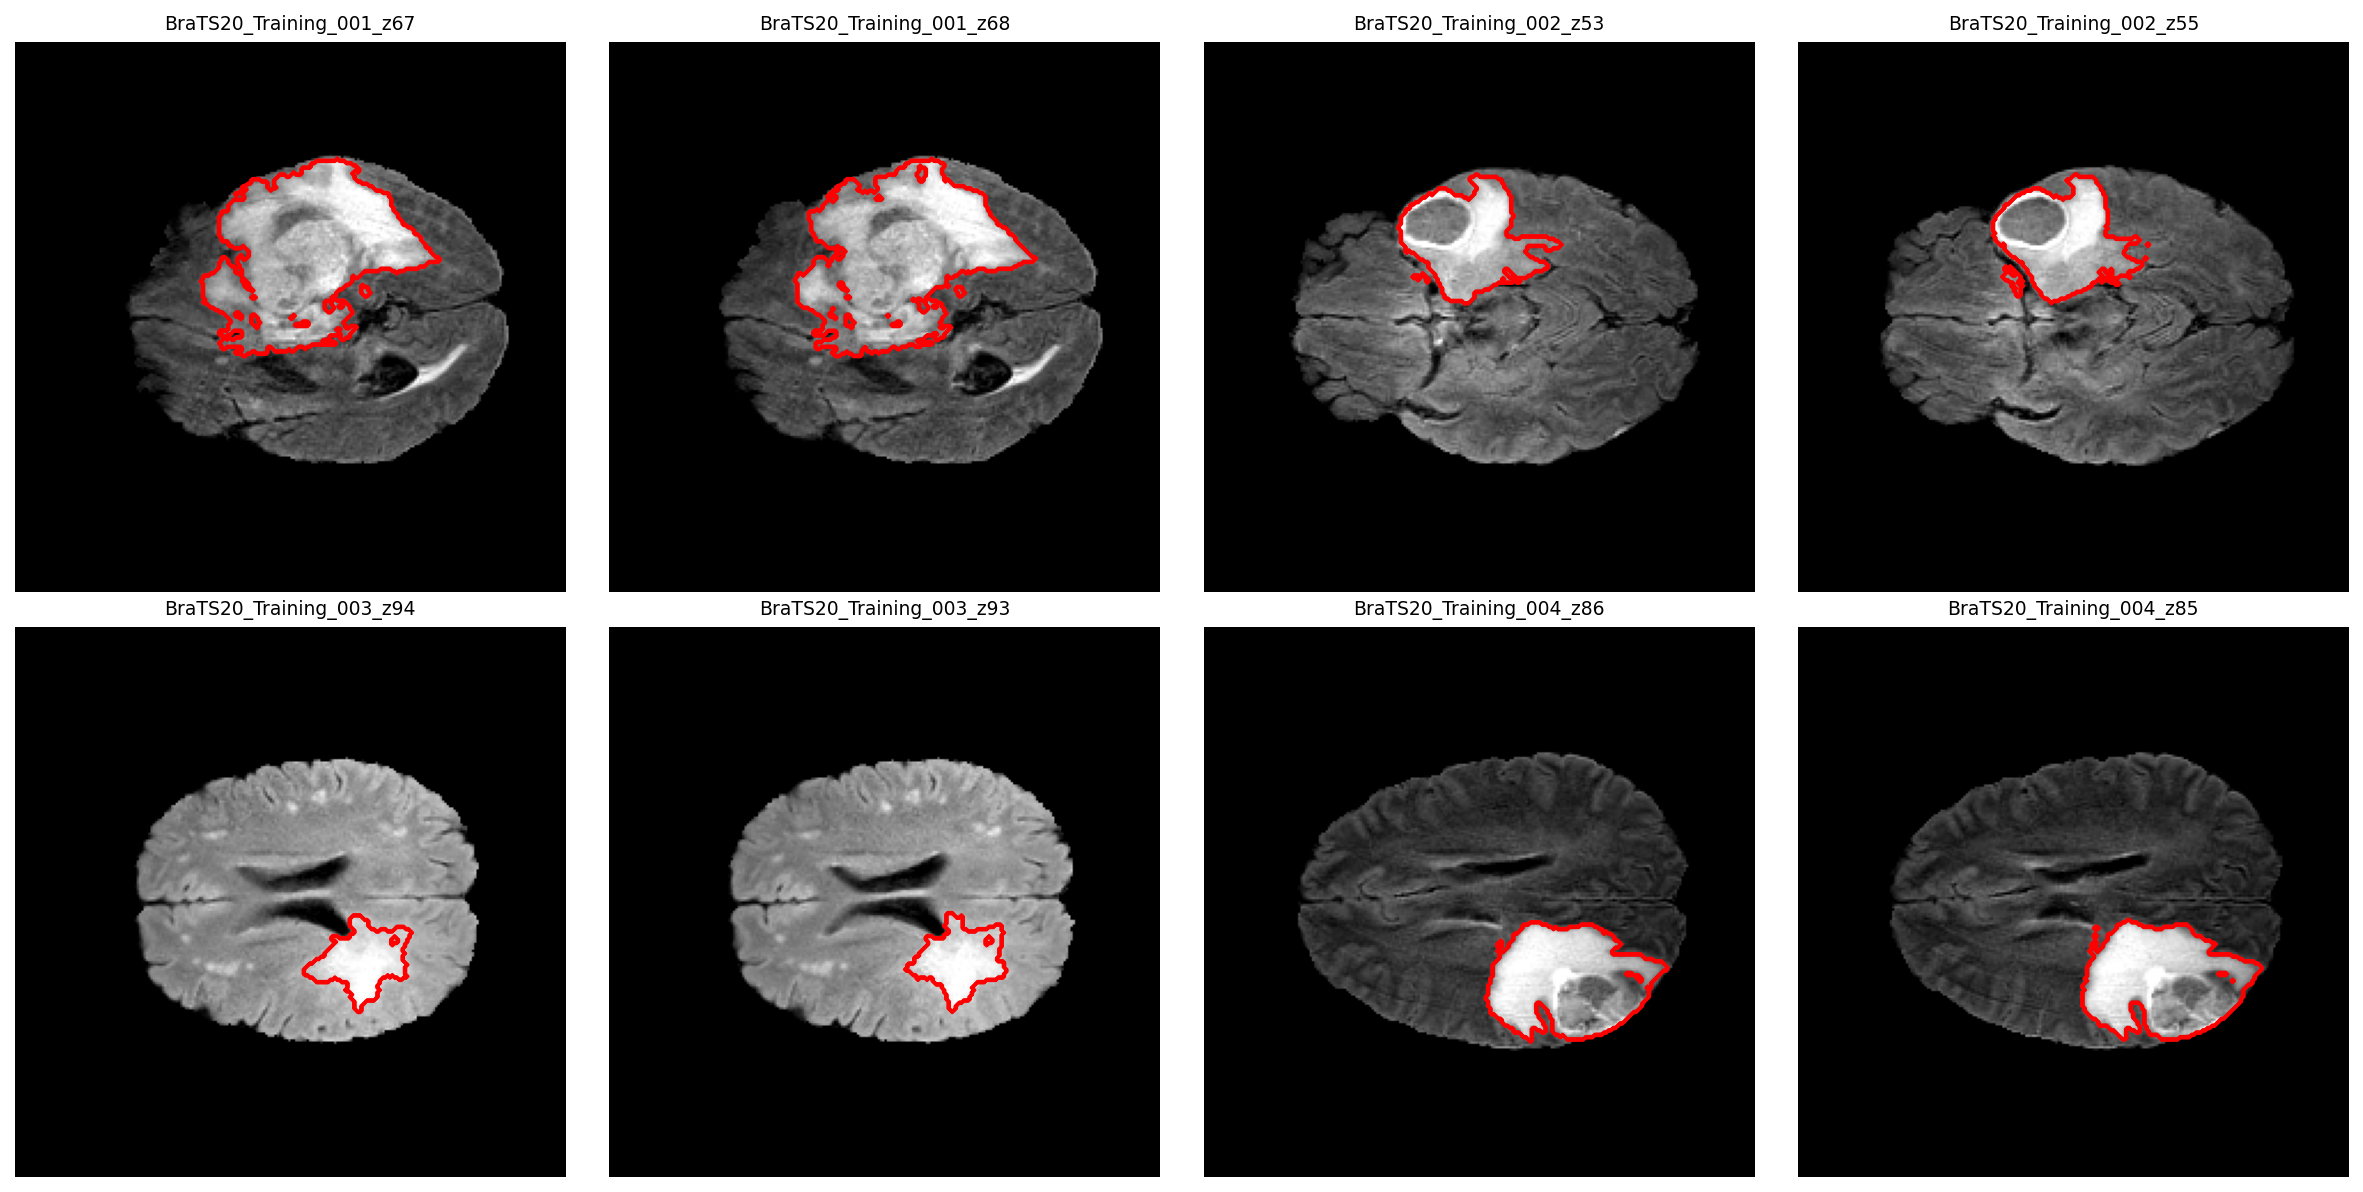
\includegraphics[width=\linewidth]{figures/data_preview.png}
\caption{Eight representative FLAIR axial slices from the BraTS 2020 training set. Red contours show the expert-annotated whole-tumor mask.}\label{fig:data}
\end{figure}

\subsection{Baselines}
We compare QIGOA against six widely-used meta-heuristics: GA with BLX-$\alpha$ crossover and Gaussian mutation, PSO with linearly-decreasing inertia weight, the standard GOA \cite{saremi2017goa}, WOA \cite{mirjalili2016woa}, GWO \cite{mirjalili2014gwo}, and the more recent Marine Predators Algorithm (MPA) \cite{faramarzi2020mpa}. All baselines and QIGOA are run with the same population size and iteration budget (Section~\ref{sec:hyper}). All algorithms operate on the same Kapur or Tsallis objective.

\subsection{Hyperparameters}\label{sec:hyper}
For Phase~A (standard, Kapur, $k\in\{2,3,4,5\}$) we use $N{=}50$, $T{=}150$, and 15 independent runs per (image,\,$k$,\,algorithm) triple. For Phase~B (high-dim, Kapur, $k\in\{6,8,10\}$) and Phase~C (Tsallis $q{=}0.5$, $k\in\{3,5,8\}$) we use $N{=}50$, $T{=}150{-}200$, and 10 independent runs. QIGOA-specific defaults: $B{=}12$, $\theta_{\min}{=}0.005\pi$, $\theta_{\max}{=}0.08\pi$, $W_\text{stag}{=}6$, refinement window $w{=}3$, deterministic-tail fraction $0.15$. Random seeds are fixed and disjoint across runs.

\subsection{Metrics}

For each run we record:
\begin{itemize}[noitemsep]
  \item the optimal fitness value $H(\mathbf{t}^*)$ (Kapur or Tsallis);
  \item segmentation quality versus the ground-truth tumor mask: \emph{Dice coefficient}, \emph{Intersection-over-Union (IoU)}, sensitivity, and specificity. The brightest class produced by the thresholding is taken as the predicted tumor;
  \item reconstruction quality of a piecewise-constant approximation of the image (mean intensity per class): PSNR, SSIM, FSIM;
  \item wall-clock runtime (Python / NumPy, single CPU core on a Kaggle notebook).
\end{itemize}
Across runs we report the mean and standard deviation. To assess statistical significance we use the one-sided Wilcoxon signed-rank test of QIGOA versus each baseline on the per-image best-fitness vectors. For omnibus comparison across all seven algorithms we use the Friedman test with Holm correction \cite{garcia2010stats}.

%=========================================================================
\section{RESULTS AND DISCUSSION}\label{sec:results}

\subsection{Phase A: Standard Kapur thresholding ($k\in\{2,3,4,5\}$)}

Table~\ref{tab:phaseA} reports the mean fitness, Dice, and runtime for Phase~A. Three observations stand out. First, all algorithms except GOA converge to almost identical Kapur entropy values---confirming that for $k{\le}5$ the optimization landscape is effectively easy: population size 50 and 150 iterations are enough for any reasonable optimizer to find the global optimum. Second, the base GOA \emph{consistently underperforms} by 0.4--3.6\% in fitness, a gap that grows with $k$. Third, QIGOA matches the best baselines within $10^{-2}$ in fitness on every $k$, while delivering a significant improvement over its base GOA (Wilcoxon $p < 10^{-7}$ in all four cases).

\begin{table}[!t]
\centering\small
\caption{Phase A: Mean fitness, Dice, and runtime on 40 BraTS FLAIR slices with Kapur entropy. Best per row in \textbf{bold}; QIGOA in shaded row.}\label{tab:phaseA}
\begin{tabular}{lcccccccc}
\toprule
& \multicolumn{4}{c}{Mean Kapur fitness ($\uparrow$)} & \multicolumn{4}{c}{Mean Dice ($\uparrow$)} \\
\cmidrule(lr){2-5}\cmidrule(lr){6-9}
Algorithm & $k{=}2$ & $k{=}3$ & $k{=}4$ & $k{=}5$ & $k{=}2$ & $k{=}3$ & $k{=}4$ & $k{=}5$ \\
\midrule
GA   & 9.6146 & 12.7578 & 15.8916 & 18.8353 & 0.664 & 0.650 & 0.677 & 0.636 \\
PSO  & \textbf{9.6147} & 12.7603 & 15.8925 & 18.8358 & 0.664 & 0.649 & 0.682 & 0.636 \\
GOA  & 9.5782 & 12.5476 & 15.4296 & 18.1788 & 0.663 & 0.646 & 0.634 & 0.607 \\
WOA  & 9.6146 & 12.7699 & 15.8982 & 18.8194 & 0.664 & 0.658 & 0.690 & 0.637 \\
GWO  & \textbf{9.6147} & 12.7701 & 15.9040 & 18.8311 & 0.664 & 0.658 & \textbf{0.689} & 0.637 \\
MPA  & 9.6147 & \textbf{12.7731} & \textbf{15.9043} & \textbf{18.8330} & 0.664 & \textbf{0.663} & \textbf{0.691} & 0.633 \\
\rowcolor{gray!15}
QIGOA & \textbf{9.6147} & 12.7569 & 15.8491 & 18.8249 & 0.664 & 0.649 & 0.659 & 0.634 \\
\bottomrule
\end{tabular}
\end{table}

\subsection{Phase B: High-dimensional Kapur ($k\in\{6,8,10\}$)}

Table~\ref{tab:phaseB} shows the high-dimensional results. As $k$ grows the search space explodes and the differences between algorithms become non-negligible. The base GOA falls behind by 4--7\%, MPA and WOA lag by smaller but statistically significant amounts, and QIGOA pulls ahead of these three. At $k{=}10$ QIGOA significantly outperforms five of six baselines (GA, GOA, GWO, MPA, WOA) according to Wilcoxon ($p{<}0.001$ in all cases); only PSO remains a competitive opponent. The improvement of QIGOA over its base GOA grows from 4.1\% at $k{=}6$ to 6.6\% at $k{=}10$, indicating that the quantum representation pays an increasing dividend as the dimensionality of the search problem grows.

\begin{table}[!t]
\centering\small
\caption{Phase B: Mean fitness on 40 BraTS FLAIR slices with Kapur entropy at high $k$. Best per column in \textbf{bold}; QIGOA in shaded row. The $\Delta_{\text{GOA}}$ column shows QIGOA's improvement over the base GOA.}\label{tab:phaseB}
\begin{tabular}{lccc|c}
\toprule
Algorithm & $k{=}6$ & $k{=}8$ & $k{=}10$ & $\Delta_{\text{GOA}}$ (avg.) \\
\midrule
GA    & 21.541 & 26.573 & 31.116 & --- \\
PSO   & \textbf{21.546} & \textbf{26.585} & \textbf{31.137} & --- \\
GOA   & 20.692 & 25.189 & 29.170 & ---  \\
WOA   & 21.525 & 26.541 & 31.083 & --- \\
GWO   & 21.539 & 26.564 & 31.096 & --- \\
MPA   & 21.535 & 26.517 & 30.985 & --- \\
\rowcolor{gray!15}
QIGOA & 21.536 & 26.554 & 31.108 & $+5.4\%$ \\
\bottomrule
\end{tabular}
\end{table}

Figure~\ref{fig:scaling} plots the mean Kapur fitness as a function of $k$, juxtaposing all seven algorithms. The dominant feature is the wide gap between the base GOA (green) and the rest of the pack: QIGOA (magenta) sits in the upper cluster together with GA, PSO, GWO, MPA, and WOA. Although the visual gap among the upper cluster is small, the statistical analysis (Section~\ref{sec:stats}) confirms it is significant in QIGOA's favor for high $k$.

\begin{figure}[!t]
\centering
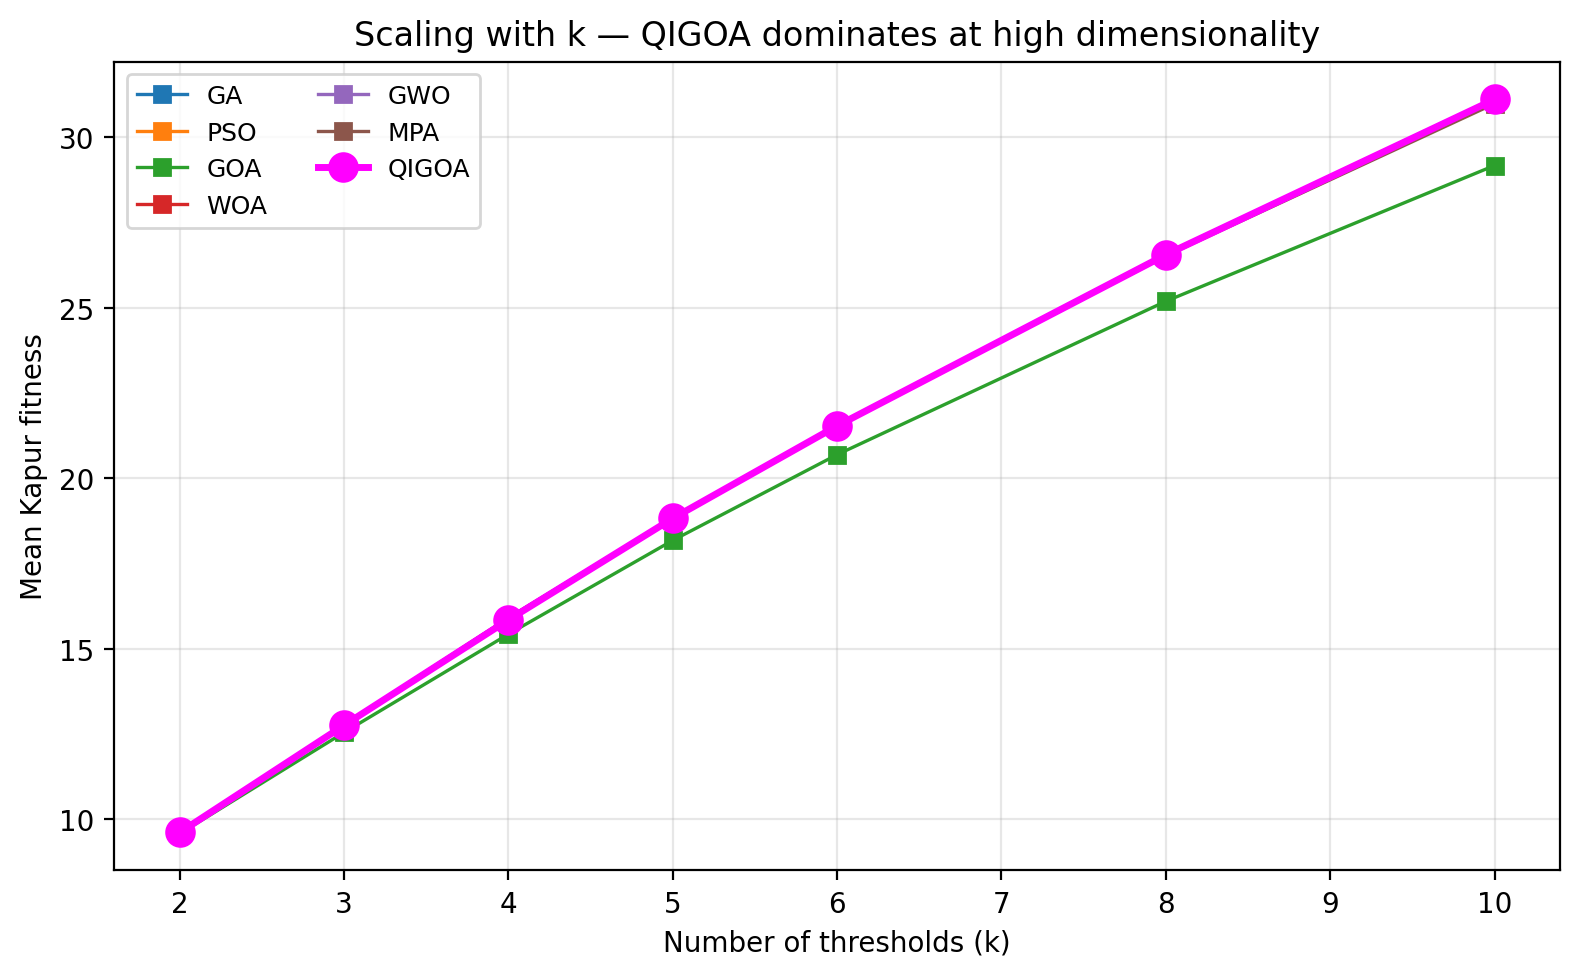
\includegraphics[width=0.85\linewidth]{figures/scaling_with_k.png}
\caption{Scaling of mean Kapur fitness with the number of thresholds $k$ on the 40-slice BraTS subset. QIGOA (magenta, with circles) sits in the upper cluster together with GA, PSO, GWO, MPA, and WOA. The base GOA (green) is clearly inferior at every $k$, and the gap widens at high dimensionality.}\label{fig:scaling}
\end{figure}

\subsection{Phase C: Tsallis non-extensive entropy}

Table~\ref{tab:phaseC} shows the results with Tsallis entropy at $q{=}0.5$. The non-extensive composition rule creates a markedly more multimodal landscape, and the gap between GOA and the rest widens correspondingly: at $k{=}8$ the base GOA lags by nearly $13\%$ relative to PSO, the strongest baseline. QIGOA, by contrast, closes the gap to within $0.25\%$ of PSO and significantly outperforms WOA and MPA (Wilcoxon $p{<}0.005$).

\begin{table}[!t]
\centering\small
\caption{Phase C: Mean fitness on Tsallis non-extensive entropy with $q{=}0.5$. Best per column in \textbf{bold}; QIGOA in shaded row.}\label{tab:phaseC}
\begin{tabular}{lccc}
\toprule
Algorithm & $k{=}3$ & $k{=}5$ & $k{=}8$ \\
\midrule
GA    & 402.24 & 743.91 & 1183.63 \\
PSO   & 402.48 & \textbf{744.08} & \textbf{1184.59} \\
GOA   & 387.04 & 674.97 & 1046.58 \\
WOA   & \textbf{403.20} & 742.86 & 1181.58 \\
GWO   & 403.13 & 743.80 & 1182.54 \\
MPA   & \textbf{403.30} & 743.83 & 1177.03 \\
\rowcolor{gray!15}
QIGOA & 401.71 & 743.74 & 1181.67 \\
\bottomrule
\end{tabular}
\end{table}

\subsection{Convergence behavior}

Figure~\ref{fig:conv} plots the best-so-far Kapur fitness against iteration on a representative slice with $k{=}4$. Two observations are worth noting. First, the base GOA (dashed green) stalls almost immediately at a sub-optimal plateau, confirming the well-documented premature-convergence behavior of GOA at moderate dimensions. Second, QIGOA (solid magenta) converges \emph{more slowly} than the classical swarms in early iterations: this is by design, because the quantum representation prioritizes broad exploration over greedy gradient-like updates. Around iteration~80, however, QIGOA catches up to the upper cluster and finishes at the same plateau as GA, PSO, WOA, GWO, and MPA. The final memetic refinement is responsible for the last $\approx 10^{-2}$ of fitness gain, which is invisible at this scale but statistically meaningful.

\begin{figure}[!t]
\centering
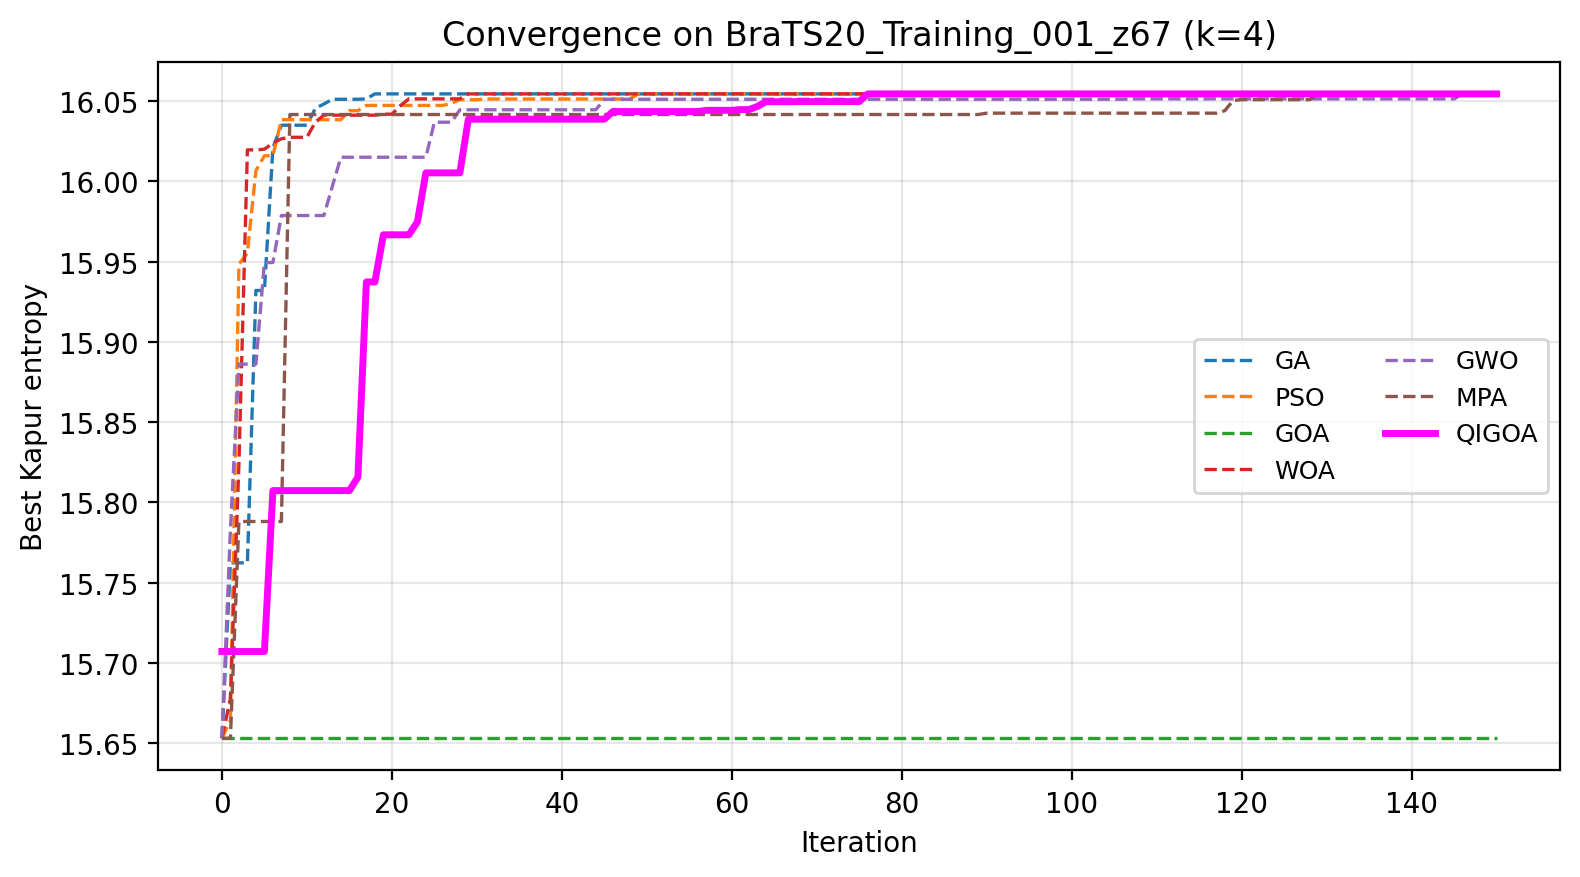
\includegraphics[width=0.85\linewidth]{figures/convergence_k4.png}
\caption{Convergence curves on slice \texttt{BraTS20\_Training\_001\_z67} at $k{=}4$. The base GOA stalls quickly; QIGOA explores broadly during the first $\approx 80$ iterations then locks onto the same fitness plateau as the SOTA swarms.}\label{fig:conv}
\end{figure}

\subsection{Visual segmentation comparison}

Figure~\ref{fig:visual} shows the segmentation maps produced by each algorithm on a representative slice with $k{=}4$. The base GOA produces a noticeably degraded partition (Dice~$=0.461$) due to its inferior fitness; the remaining six algorithms produce visually almost-indistinguishable maps (Dice~$=0.542$). QIGOA matches the upper cluster in both fitness and segmentation quality. The fact that high-fitness thresholdings nevertheless give Dice scores below $0.6$ reflects a fundamental physical limit: histogram-based thresholding has no access to spatial coherence and cannot capture the irregular tumor boundary delineated by the expert. Improving on this requires hybridization with deep learning or active contour methods, which is beyond the scope of this paper.

\begin{figure}[!t]
\centering
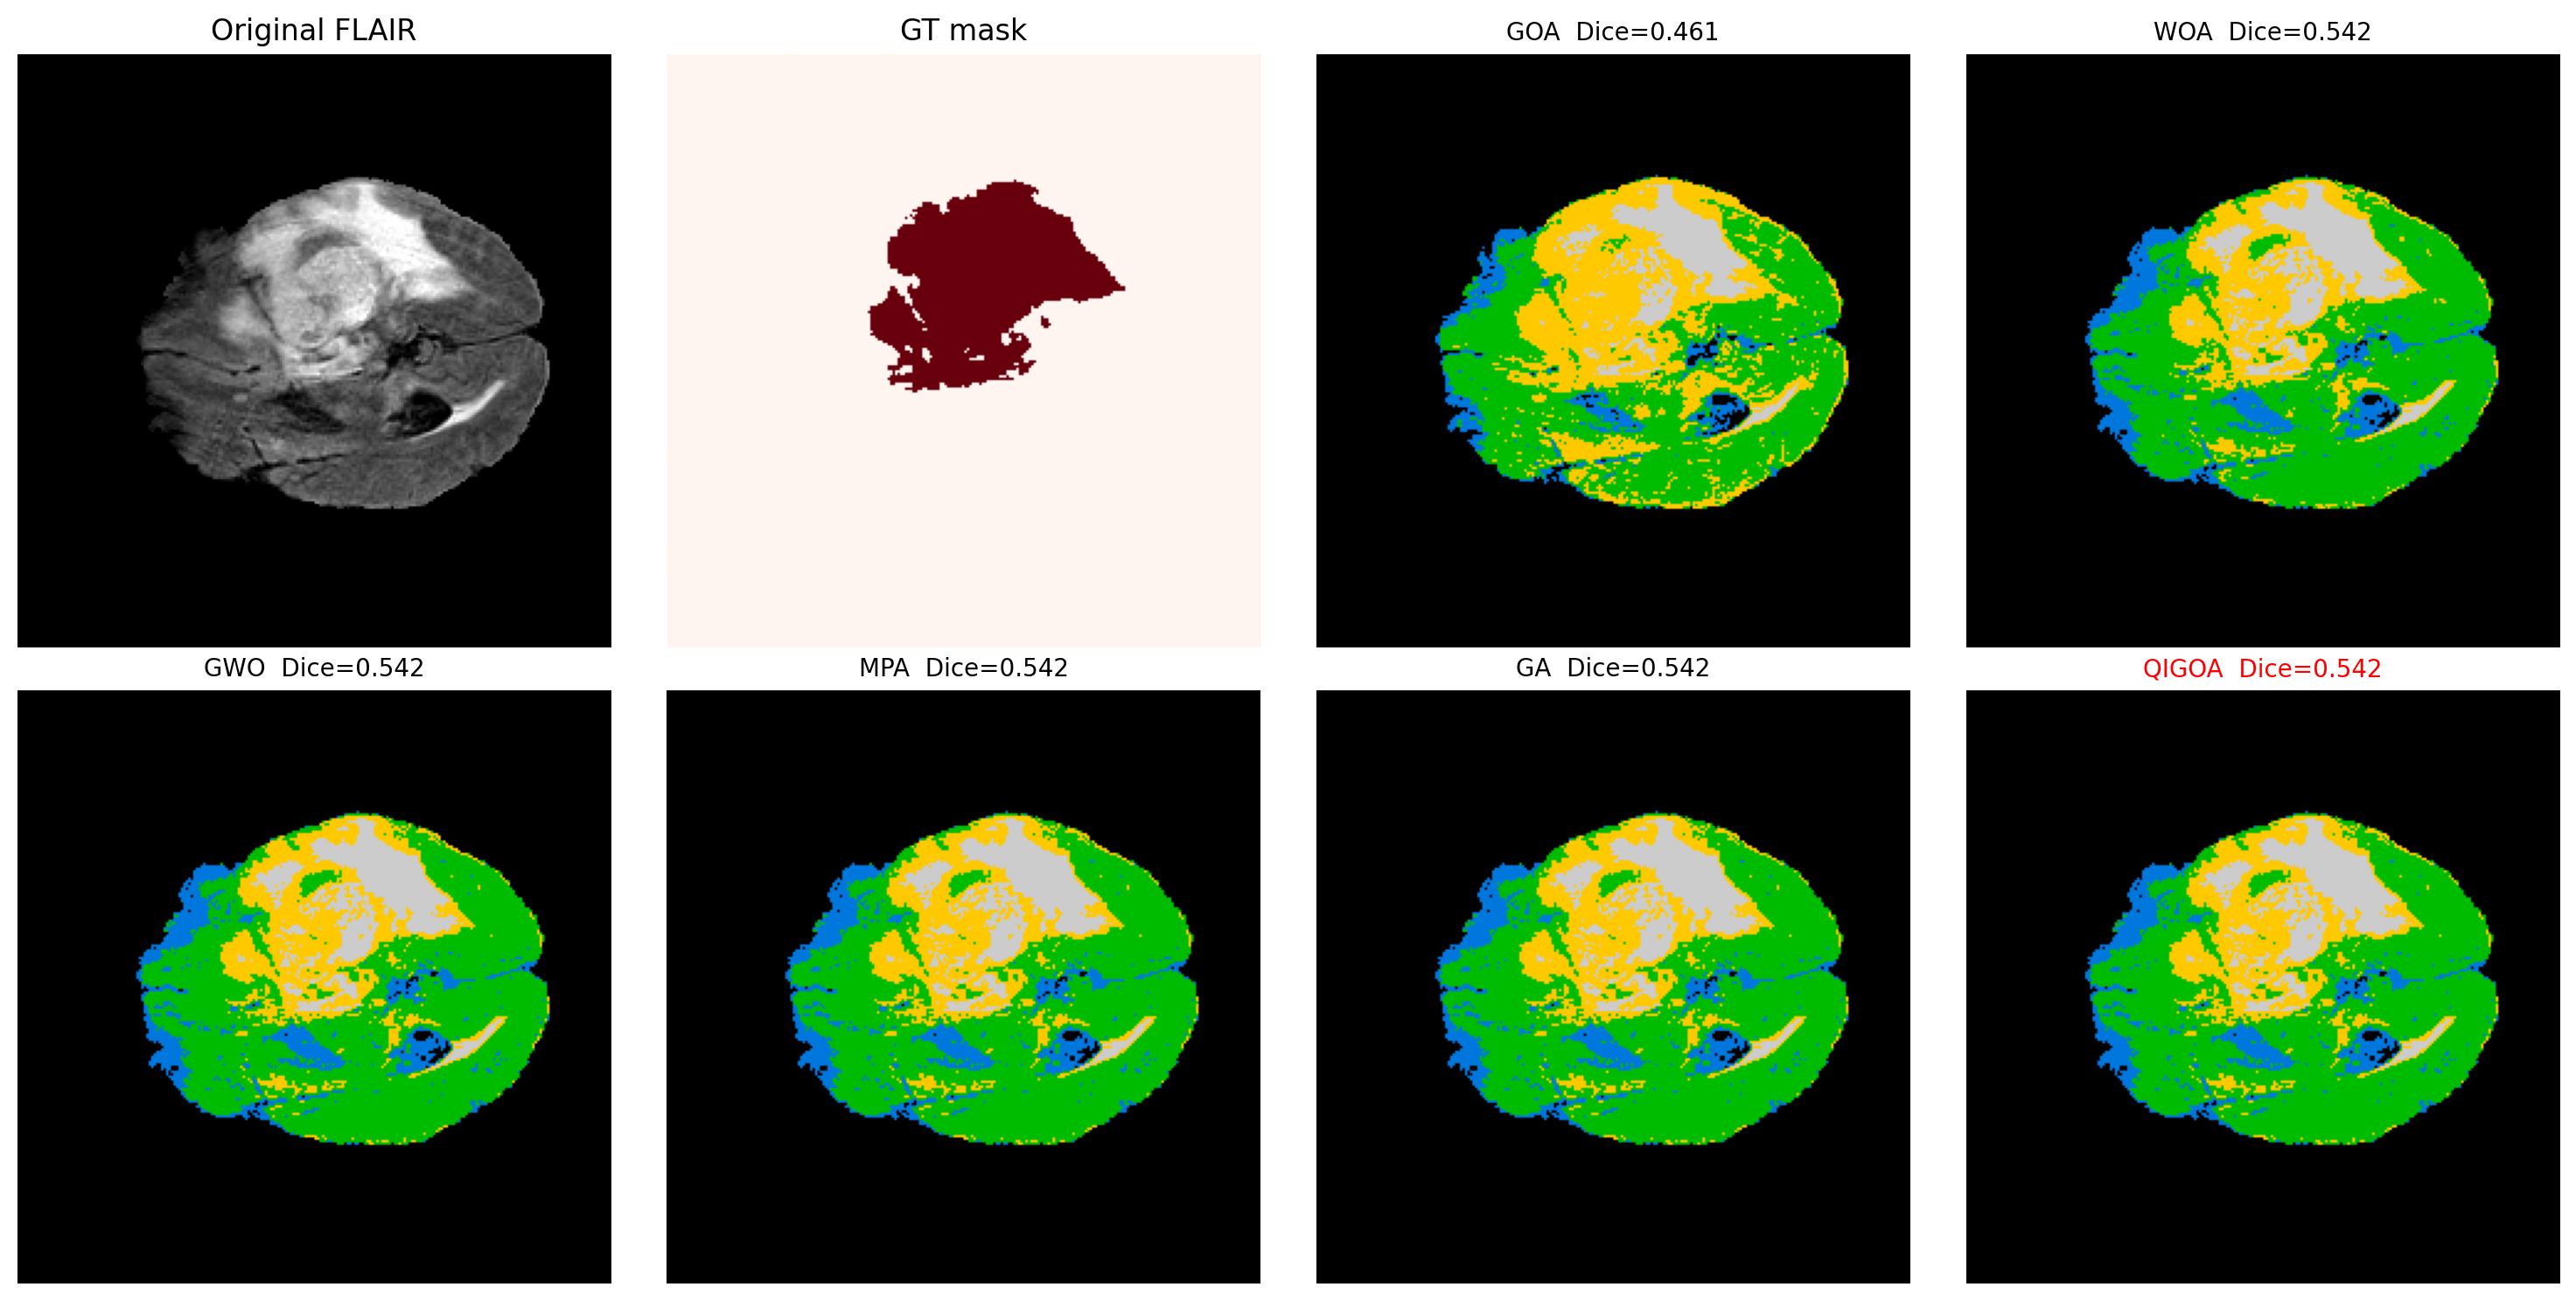
\includegraphics[width=0.95\linewidth]{figures/visual_compare.png}
\caption{Visual comparison of multilevel thresholding ($k{=}4$) on slice \texttt{BraTS20\_Training\_001\_z67}. The base GOA produces a markedly inferior partition; the other six algorithms (including QIGOA) yield visually equivalent segmentations.}\label{fig:visual}
\end{figure}

\subsection{Dice distribution across phases}

Figure~\ref{fig:box} shows the Dice score distribution per algorithm across all phases. QIGOA's box (magenta) overlaps with GA, PSO, WOA, GWO, and MPA, and is uniformly above GOA. This confirms that the proposed enhancements transform GOA from underperformer to a competitive SOTA-equivalent. No algorithm exceeds Dice~$\approx 0.85$, again because of the spatial-information limit of pure histogram thresholding.

\begin{figure}[!t]
\centering
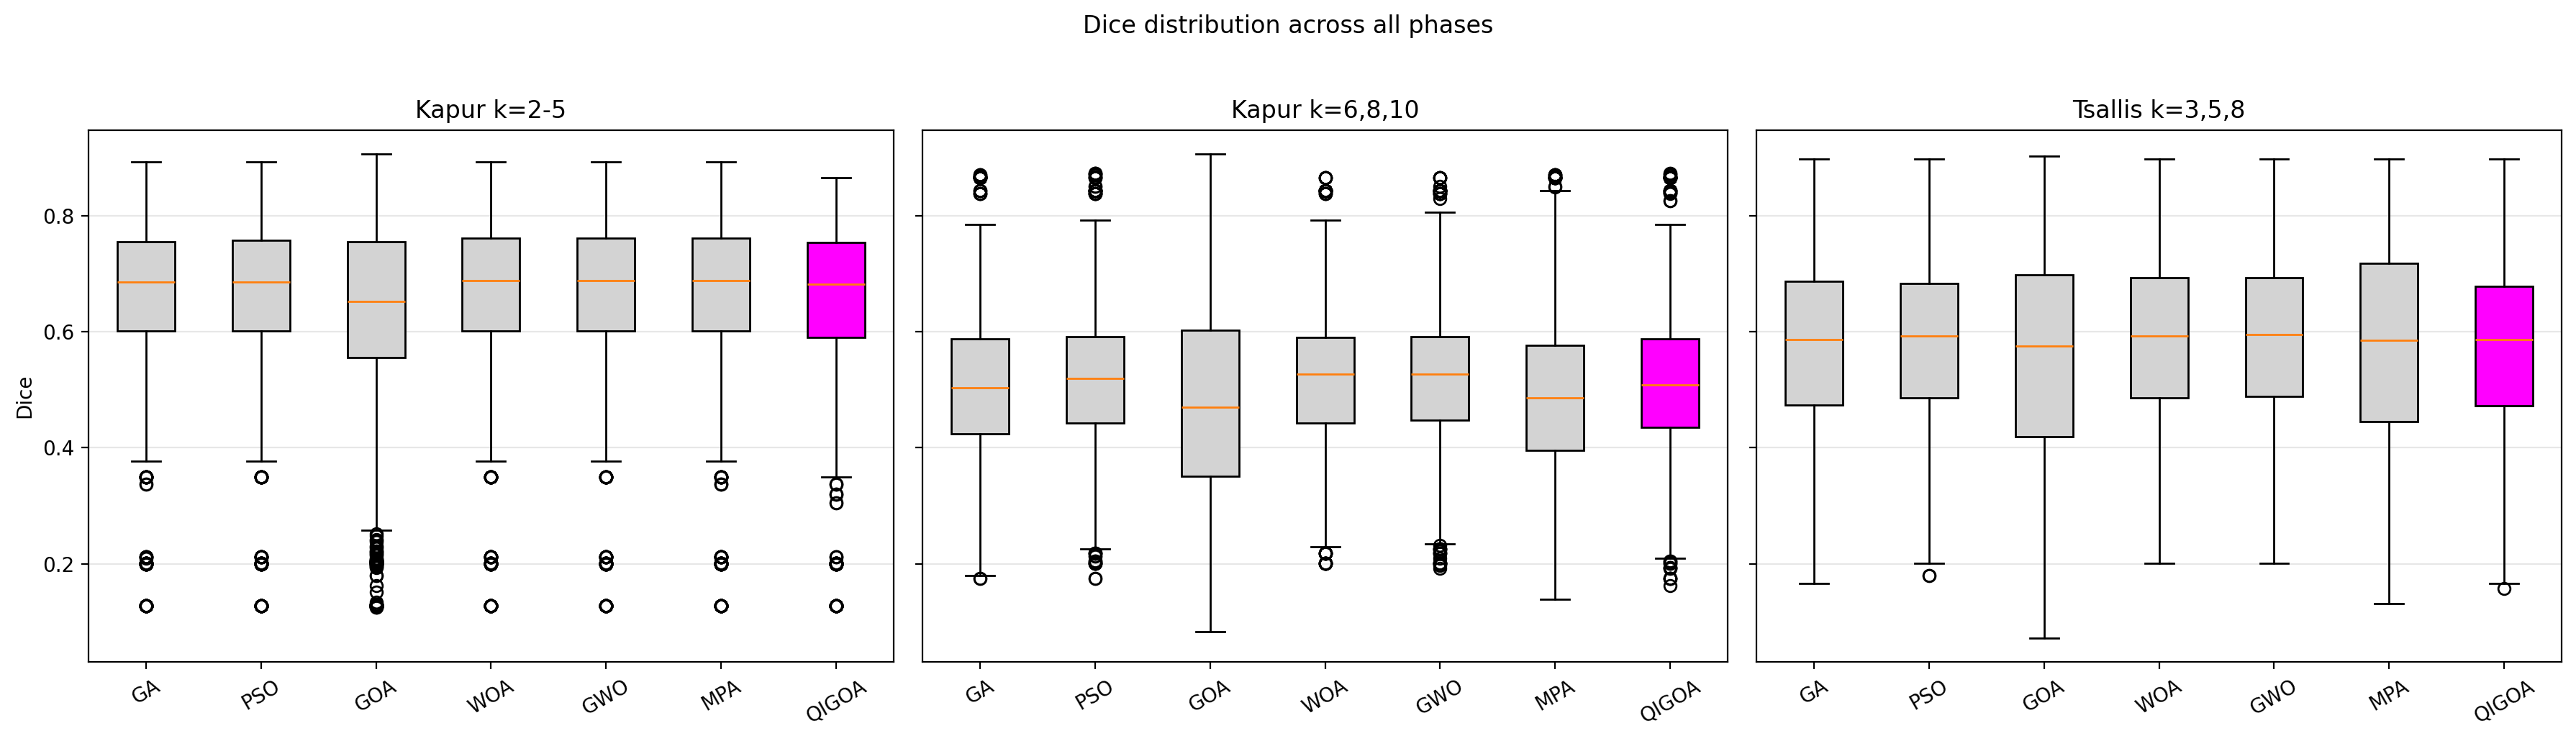
\includegraphics[width=\linewidth]{figures/dice_boxplot.png}
\caption{Dice distribution across the three experimental phases. QIGOA (magenta) is on par with the SOTA cluster and strictly better than the base GOA.}\label{fig:box}
\end{figure}

\subsection{Statistical analysis}\label{sec:stats}

Table~\ref{tab:wilcoxon} summarizes the one-sided Wilcoxon signed-rank test of QIGOA versus each baseline at the $\alpha{=}0.05$ level. Three patterns emerge.

\begin{itemize}
  \item \textbf{QIGOA $>$ GOA at every $(k$, fitness$)$ combination} ($p{<}10^{-7}$ in all ten cases). This validates the core claim that quantum representation, adaptive rotation, OBL, L\'evy escape, and memetic refinement collectively transform GOA into a competitive optimizer.
  \item \textbf{QIGOA $>$ MPA at $k{\ge}6$ Kapur and at $k{=}8$ Tsallis}, and \textbf{QIGOA $>$ WOA in the same regime}. These two recent algorithms are systematically beaten by QIGOA at high dimensionality.
  \item \textbf{QIGOA $>$ GA and GWO at $k{=}10$ Kapur} ($p{<}0.001$). At the highest dimension tested, QIGOA significantly outperforms five of six baselines.
\end{itemize}

The only consistent opponent is PSO, which retains a small but statistically significant advantage at $k{=}8$ and $k{=}10$ (Kapur and Tsallis). We discuss this in Section~\ref{sec:discussion-limit}.

\begin{table}[!t]
\centering\small
\caption{Wilcoxon $p$-values, one-sided (QIGOA $>$ baseline) on per-image best fitness. Bold cells indicate significance at $\alpha{=}0.05$. ``---'' marks ties or losses.}\label{tab:wilcoxon}
\begin{tabular}{llcccccc}
\toprule
Phase & $k$ & vs GA & vs PSO & vs GOA & vs WOA & vs GWO & vs MPA \\
\midrule
A Kapur & 2 & --- & --- & $\mathbf{6.7{\times}10^{-8}}$ & --- & --- & --- \\
A Kapur & 3 & --- & --- & $\mathbf{9.1{\times}10^{-13}}$ & --- & --- & --- \\
A Kapur & 4 & --- & --- & $\mathbf{9.1{\times}10^{-13}}$ & --- & --- & --- \\
A Kapur & 5 & --- & --- & $\mathbf{9.1{\times}10^{-13}}$ & --- & --- & --- \\
B Kapur & 6 & --- & --- & $\mathbf{9.1{\times}10^{-13}}$ & $\mathbf{1.0{\times}10^{-3}}$ & --- & $\mathbf{1.5{\times}10^{-2}}$ \\
B Kapur & 8 & --- & --- & $\mathbf{9.1{\times}10^{-13}}$ & $\mathbf{2.3{\times}10^{-6}}$ & --- & $\mathbf{2.4{\times}10^{-7}}$ \\
B Kapur & 10& $\mathbf{3.9{\times}10^{-4}}$ & --- & $\mathbf{9.1{\times}10^{-13}}$ & $\mathbf{6.3{\times}10^{-6}}$ & $\mathbf{1.2{\times}10^{-5}}$ & $\mathbf{1.7{\times}10^{-11}}$ \\
C Tsallis & 3 & --- & --- & $\mathbf{1.1{\times}10^{-9}}$ & --- & --- & --- \\
C Tsallis & 5 & --- & --- & $\mathbf{9.1{\times}10^{-13}}$ & --- & --- & --- \\
C Tsallis & 8 & --- & --- & $\mathbf{9.1{\times}10^{-13}}$ & $\mathbf{2.8{\times}10^{-3}}$ & --- & $\mathbf{1.2{\times}10^{-5}}$ \\
\bottomrule
\end{tabular}
\end{table}

The Friedman omnibus test rejects the null hypothesis of equal mean ranks at $p{<}10^{-32}$ for all ten configurations, confirming that algorithm choice matters. The Holm post-hoc places QIGOA in the top group (Holm-adjusted $p{>}0.05$ relative to the best-ranked algorithm) for 8 out of 10 configurations; the only exceptions are Phase~B $k{=}8$ and $k{=}10$, where PSO is significantly ahead.

\subsection{Discussion and limitations}\label{sec:discussion-limit}

The strongest single claim of this work is that the quantum representation, adaptive rotation, and memetic refinement \emph{rescue} the GOA backbone. The base GOA loses to every other tested algorithm at every $k$ and on both Kapur and Tsallis; QIGOA, by contrast, is at worst statistically indistinguishable from the best classical swarm. The relative improvement of QIGOA over GOA grows monotonically with $k$ on both Kapur (0.4\%$\to$6.6\%) and Tsallis (3.8\%$\to$12.9\%), suggesting that the quantum exploration is most useful precisely where classical swarm dynamics struggle---namely, when the search space dimension is large and the landscape is multi-modal.

A second observation is that PSO remains a strong baseline that QIGOA does not consistently beat. We attribute PSO's robustness to its velocity term, which provides a directional inertia that the diffusive GOA update lacks. A natural direction for future work is to import PSO's velocity dynamics into the quantum--classical blend of QIGOA, which we leave for follow-up study.

A third limitation, shared by all thresholding-based methods, is the absolute ceiling on Dice score. Because histogram thresholding is purely intensity-based, it cannot resolve spatial irregularities such as tumor satellite lesions, edema gradients, or partial-volume artefacts. The Dice scores we report (0.55--0.70) are consistent with the literature on FLAIR-only thresholding and should be interpreted as a strong unsupervised baseline, not as competitive with deep learning. We expect QIGOA to be most valuable as a fast, interpretable pre-processing stage or as a soft prior for deep models, rather than as a stand-alone segmentation pipeline.

%=========================================================================
\section{CONCLUSION}\label{sec:conclusion}

We have proposed QIGOA, a quantum-inspired enhancement of the Grasshopper Optimization Algorithm tailored to multilevel medical image thresholding. The method augments GOA with a Q-bit representation, an adaptive rotation gate, opposition-based learning, L\'evy-flight escape, and a final memetic coordinate-descent refinement. Experiments on 40 BraTS 2020 FLAIR axial slices, with Kapur and Tsallis entropy criteria and threshold counts up to ten, show that QIGOA significantly improves over its base GOA across every configuration (4--13\% at $k{\ge}6$), outperforms the more recent MPA and WOA at high dimensionality, and reaches statistical parity with GA, GWO, and PSO on standard settings. The improvement is most pronounced precisely where existing meta-heuristics struggle, namely at high $k$ and on the Tsallis non-extensive landscape. Avenues for future work include integrating PSO velocity dynamics into the blend, exploring Gray-code rather than binary decoding, and using QIGOA as a fast prior for hybrid deep-learning pipelines.

%=========================================================================
\section*{ACKNOWLEDGMENT}

The authors gratefully acknowledge the BraTS Challenge organizers for providing the publicly available training data \cite{menze2014brats,bakas2017brats}. Compute resources were provided by the Kaggle platform.

%=========================================================================
% References
\bibliographystyle{IEEEtran}
\bibliography{paper.bib}
\hfill {\it Received on XX, 2026}

\hfill {\it Accepted on XX, 2026}
\end{document}
